\chapter{SM-02}
Boltzman entrophy relation: $S=K \ln \Omega$\\
striling approximation: $\ln n !=n \ln n-n$\\
Number of microstates: 
$\Omega_{M B}=\underset{i}{\pi}\left(g_{i}\right)^{n_{i}}$\\
$\Omega_{B E}=\underset{i}{\pi}\frac{\left(n_{i}+g_{i}-1\right) !}{n_{i} !(g i-1) !}$\\
${ }^{\Omega_{F D}}=\underset{i}{\pi}{g i }\  C_{n_{i}}$\\
$g_{i} \rightarrow$ degeneracy\\
$n_{i} \rightarrow$ identical Particles\\
Energy distribution function :$f(E)=\frac{n_{i}}{g_{i}}$
Q.The number of ways in which $N$ identical bosons can distributed in two energy levels is 
 \begin{tasks}(4)
	\task[\textbf{a.}] $N+1$
	\task[\textbf{b.}]$N(N-1) \mid 2$
	\task[\textbf{c.}]$N(N+1) \mid 2$
	\task[\textbf{d.}]$N$ 
\end{tasks}
\begin{answer}
	\begin{align*}
	\Omega&=N_ {C_n}=\frac{N !}{n !(N-n) !}\hspace{2cm}\underset{\text{-------------- }e}{n}\\
	\text { entropy }(s)&=k \ln \Omega=k \ln \frac{N !}{n !(N-n) !}\hspace{1.1cm}\underset{\text{-------------- } 0}{(N-n)}\\
	\operatorname{s\alpha } &\ln \frac{N !}{n !(N-n) !}
	\end{align*}
		So the correct answer is \textbf{Option (d)}
\end{answer}
\begin{note}
	Probability will be maximum for equal distribution.
\end{note}
Q. Let $N_{M B}, N_{B E}, N_{F D}$ denote the number of ways in which two particles can be distributed in two energy states according to maxwell-Boltzmann, Bose-Einstein \& fermi-Dirac statistics respectively. Then $N_{M B}: N_{B E}: N_{F D}$ is:
 \begin{tasks}(4)
	\task[\textbf{a.}]$4: 3: 1$
	\task[\textbf{b.}] $4: 2: 3$
	\task[\textbf{c.}]$4: 3: 3$
	\task[\textbf{d.}] $4: 3: 2$
\end{tasks}
\begin{answer}
	\begin{align*}
	\Omega_{M B}&=\left(g_{i}\right)^{n_{i}}=(2)^{2} \Rightarrow 4 \\
	\Omega_{B E}&=\frac{\left(n_{i}+g_{i}-1\right) !}{n_{i} !((-i-1) !}=\frac{(2+2-1) !}{2 !(2-1) !}=\frac{3 !}{2 !}=3\\
	\Omega_{F D}&=g i C_{n_{i}}=\frac{2 !}{2 ! 1 !}=1\\
	&4:3:1
	\end{align*}
	So the correct answer is \textbf{Option (a)}
\end{answer}
Relative Probability: \\
$$r=\frac{P_1}{P_2}=\frac{\text{Probability of finding particle in same state}}{\text{Probability of finding particle in different state.}}$$
$r_{B E}: r_{M B}: r_{F \cdot D}=1: 1 / 2: 0$\\
$\Rightarrow U_{B E} \leqslant U_{M B} \leqslant U_{F D} \Rightarrow P_{B E} \leqslant P_{M B} \leqslant P_{F D}$ \\
Q If $N$ particle are to be distributed into two groups such that group i contain $n_1$ particles and group two contains $n_2$ particles, and $N=n_1+n_2$ Find the number of ways of distribution?
\begin{answer}
	\begin{align*}
	\Omega&={ }^{N} C_{n_{1}} \text { or }{ }^{N} C_{n_{2}} 4 N=n_{1}+n_{2}\\
	N_{C_{n_{i}}}&=\frac{N !}{n_{1} !(N-n) !}=\frac{N !}{n_{1} ! n_{2} !}\\
	&\text{similaarly, for $ni$ particles}\\
	\Omega&=\frac{N!}{n_1!n_2!.......n_i!}
	\end{align*}
\end{answer}
Q. A system has energy levels $E_{0}, 2 E_{0}, 3 E_{0}, \ldots .$ where the excited states are triphy generate four non-interacting bosons are placed in this system. If the total energy og these bosons is $5E_0$ the number of microstates is:
 \begin{tasks}(4)
	\task[\textbf{a.}]2
	\task[\textbf{b.}]3
	\task[\textbf{c.}]4
	\task[\textbf{d.}] 5
\end{tasks}
\begin{answer}
	\begin{figure}[H]
		\centering
		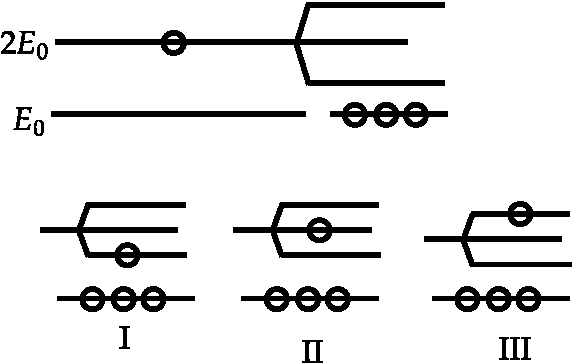
\includegraphics[height=4cm,width=6cm]{SP-12}
	\end{figure}
	So the correct answer is \textbf{Option (b)}
\end{answer}
\textbf{Phase Space}:(Position + momentum) space\\
volume of single phase cell: $d \tau=h^{f} \quad f \rightarrow D O F$\\
allowed vol. of phace space: $\int d^{3} q \int d^{3} p$\\
$$
V_{p} \Rightarrow V \times \frac{4}{3} \pi p^{3}\text{( for 3-Dim).}
$$
\textbf{Non-Relativistic Free Particle: }$E=p^2/2m$\\
\renewcommand*{\arraystretch}{1.8}
 \begin{tabular}{|p{4cm}|p{4cm}|p{4cm}|}
 	\hline
 3-Dimensional&2-Dimensional&1-Dimensional\\\hline
 $d \tau=h^{3}$&$d \tau=h^{2}$&$d \tau=h$\\\hline
 $V_{p}=V \times \frac{4}{3} \pi p^{3}$&$V_{p}=A \times \pi p^{2}$&$V_p=L\times2p$\\\hline
 $\Omega=\frac{V \cdot \frac{4}{3} \pi p^{3}}{\hbar^{3}}$&$\Omega(p)=\frac{\pi \times \pi p^{2}}{h^{2}}$&$\Omega(p)=\frac{L \times 2 p}{h}$\\\hline
 $\Omega(E)=\frac{\mu\pi V(2mE)^3}{3h^3}$&$\Omega(E)=\frac{\pi A(2mE)}{h^2}$&$\Omega(E)=\frac{2L\sqrt{2mE}}{h}$\\\hline
 $\Omega^{\prime}(E)=\frac{2 \pi V(2 m)^{3 / 2} E^{1 / 2}}{h^2}dE$&$\Omega^{\prime}(E)=\frac{2 \pi mA}{h^3}dE$&$\Omega^{\prime}(E)=\frac{L(2m)^{1/2}E^{-1/2}}{h}dE$\\\hline
 \end{tabular}
\begin{figure}[H]
	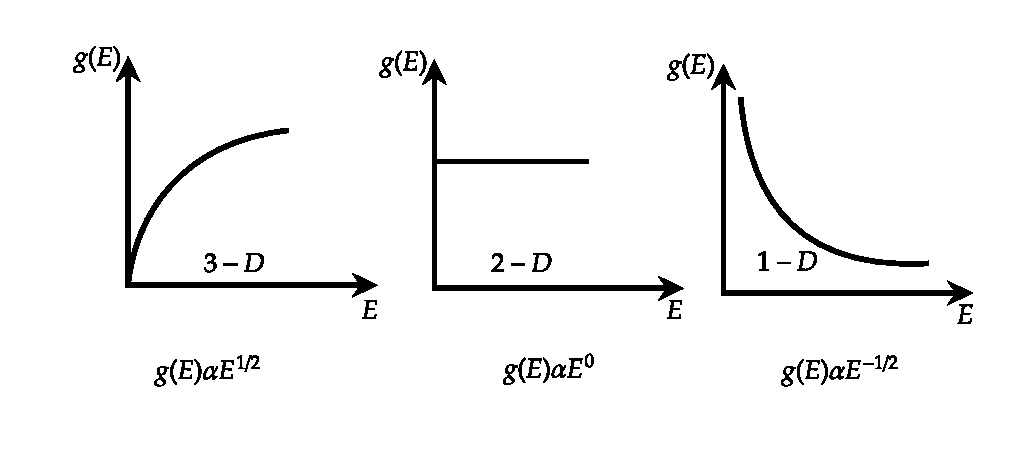
\includegraphics[height=5.5cm,width=13cm]{SP-13}
\end{figure}
\begin{exercise}
	In a classical microcanonical ensemble for a system of $N$ non-interacting particles, the fundamental volume of phase space which is regarded as "equivalent to one-microstate" is 
\end{exercise}
 \begin{tasks}(4)
	\task[\textbf{a.}] $h^{3 N}$
	\task[\textbf{b.}]$h^{2 N}$
	\task[\textbf{c.}]$h^{N}$
	\task[\textbf{d.}]$h$
\end{tasks}
\begin{answer}
	\begin{align*}
	\text{For $N$ non-interacting particles }\text { DOF }&=3 N=f\\
	\text{volume of phase space }&=h^{f}\\
	&=R^{3 N}
	\end{align*}
	So the correct answer is \textbf{Option (a)}
\end{answer}
\textbf{Extremely Relativistic Free Particle: }(E=pc)\\
\renewcommand*{\arraystretch}{1.8}
\begin{tabular}{|p{4cm}|p{4cm}|p{4cm}|}
	\hline
	3-Dimensions & 2-Dimensions & 1-Dimensions\\\hline
	$\Omega(p)=\frac{v \cdot \frac{4}{3} \pi p^{3}}{h^{3}}$&$\Omega(p)=\frac{\pi A p^{2}}{h^{2}}$&$\Omega(p)=\frac{L \times 2 p}{h}$\\
	$\Omega^{\prime}(p)=\frac{4 \pi V p^{2} d p}{h^{3}}$&$\Omega^{\prime}(p)=\frac{2 \pi A p d p}{h^{2}}$&$\Omega^{\prime}(p)=\frac{2 L d p}{h}$\\\hline
	$\Omega(E)=\frac{4 \pi V E^{3}}{3 c^{3} h^{3}}$&$\Omega(E)=\frac{A \pi E^{2}}{C^{2} n^{2}}$&$\Omega(E)=\frac{2 L E}{\hbar c}$\\
	$\Omega(E)=2 \times \frac{4 \pi v\left(E^{2}\right)}{c^{3} h^{3}} d E$&$\Omega^{\prime}(E)=\frac{2 \pi A E}{C^{2} h^{2}}$&$\Omega^{\prime}(E)=\frac{2 L}{R C} d E$\\\hline
\end{tabular}
Q. Find density of states at energy $E$ of the quantized radiation (photon) is:
 \begin{tasks}(4)
	\task[\textbf{a.}]$\frac{8 \pi v}{h^{3} c^{3}} E^{2}$
	\task[\textbf{b.}]$\frac{8 \pi V}{h^{3} c^{3}} E^{3 / 2}$
	\task[\textbf{c.}]$\frac{8 \pi V}{h^{3} c^{3}} E$
	\task[\textbf{d.}] $\frac{8 \pi V}{h^{3} c^{3}} E^{3 / 2}$
\end{tasks}
\begin{answer}
	\begin{align*}
	\Omega(p)&=\frac{V \times \frac{4}{3} \pi p^{3}}{h^{3}} \Rightarrow \Omega(E)=\frac{4 \pi V E^{3}}{3 c^{3} h^{3}}\\
	\Omega^{\prime}(E)&=\left(\frac{4 \pi V E^{2}}{c^{3} h^{3}} d E\right) \times 2\\
	\Omega^{\prime}(E)&=g(E) d E\\
	g(E)&=\frac{8 \pi V}{c^{3} h^{3}} E^{2}
	\end{align*}
	So the correct answer is \textbf{Option (a)}
\end{answer}
Q. \textbf{For free particle (with $E=ap^s$) with d-DOF: }\\
\begin{align*}
\text{Volume of sphere of radius (R) }V_{d}&=\frac{\pi^{d / 2} R^{d}}{\left(\frac{d}{2}\right) !}\\
\text{area of sphere of radius (R) }s_{d}&=\frac{2 \pi^{d / 2} R^{d-1}}{\left(\frac{d}{2}-1\right) !}\\
\text{ volume of single phase cell }d \tau&=h^{d}\\
g(E)&=\frac{g i V_{d} \pi^{d / 2}\left(\frac{1}{a}\right)^{d / s}\left(\frac{d}{s}\right) E^{(d / s-1)}}{R^{d}(d / 2) !}\\
&g(E) \propto E^{(d / s-1)}\hspace{3cm}d=DOF\\
s=1 \text{(marsless)},\quad
2 \text{(massive)}
\end{align*}
\begin{exercise}
	For an energy state $E$ of a photon gas, the density of states is proportional to 
\end{exercise}
 \begin{tasks}(4)
	\task[\textbf{a.}] $\sqrt{E}$
	\task[\textbf{b.}] $E $
	\task[\textbf{c.}]$E^{3 / 2}$
	\task[\textbf{d.}] $E^{2}$
\end{tasks}
\begin{answer}
	\begin{align*}
	D(E) &\propto E^{\left(\frac{d}{s}-1\right)}\\
	\text { For proton: } d&=3 \text { and } s=1\\
	D(E) \propto E^{3-1} &\Rightarrow D(E) \alpha E^{2}
	\end{align*}
		So the correct answer is \textbf{Option (d)}
\end{answer}
\begin{exercise}
 The number of states for a system of $N$ indentical free particles in a three dimensional space having total energy between $E$ and $E+\delta E(\delta E<<E),$ is proportional to 
\end{exercise}
 \begin{tasks}(4)
	\task[\textbf{a.}]$E^{\left(\frac{3 N}{2}-1\right)} \delta E$
	\task[\textbf{b.}]$E^{\frac{N}{2}} \delta E$
	\task[\textbf{c.}]$N E^{\frac{1}{2}} \delta E$
	\task[\textbf{d.}]$N^{N} \delta E$ 
\end{tasks}
\begin{answer}
	\begin{align*}
	D(E) &\propto E^{(d / s-1)}\\
	\text { Here } d&=3 \mathrm{~N} \text { and } s=2 \text { (massive) }\\
	D(E) &\propto E^{\left(\frac{3 N}{2}-1\right)}
	\end{align*}
		So the correct answer is \textbf{Option (a)}
\end{answer}
\begin{exercise}
 Draw phase space trajectory of linear (1-dimension) Harmonic oscillator and calculate number of microstate if particle has:\\
	a). sharp value of energy\\
	b). Energy lies between $E$ to $E+d E$
\end{exercise}
\begin{answer}
	\begin{align*}
	E&=\frac{p^{2}}{2 m}+\frac{1}{2} m \omega^2 x^{2}\\
	1&=\frac{p^{2}}{\sqrt{2 m E}}+\frac{x^{2}}{\left(\sqrt{\frac{2 E}{m \omega^2}}\right)^{2}}\\
	\text{area of ellipse }&=\pi a b\\
	\text{volume of single phase cell }&(1-D)=h\\
	\Omega(E)=\frac{\pi a b}{h}&=\frac{\pi \times \sqrt{\frac{2 E}{m \omega^2}}  \times \sqrt{2 m E}}{h}\\
	\Omega(E)&=\frac{2 \pi E}{h \omega}=\frac{E}{h \omega}\\
	\Omega^{\prime}(E)&=\frac{d E}{\hbar \omega}
	\end{align*}
\end{answer}
\begin{note}
	\begin{align*}
	\text{	maxinum valle of }&x \\
\text{	on }x-\text{axis: }p&=0 \hspace{3cm}x_{0}=\sqrt{\frac{2 E_{0}}{m \omega^{2}}}\\
	E_{0}&=0+\frac{1}{2} m u^{2} x_{0}^{2}\hspace{2cm}x_{0} \alpha \sqrt{E_{0}}\\
	\end{align*}
\end{note}